\documentclass[10pt]{article}
\usepackage{icmlko}

\icmlmeta{IP 파운데이션 월드모델}{227}{섞으면 둘 다보다 낫다}{노트 226의 분해가 정식화 하나를 제안했다. 그대로 만들었더니 실패했고, 순서를 빼니 됐다}

\begin{document}

\twocolumn[
\icmlheader

\begin{abstract}
노트 226이 \textbf{트리$-$선형(풀링) $=$ 트리$-$선형(혼자) $-$ (능형 이득
$-$ 트리 이득)}을 닫고, ``트리에 축소를 붙이면 둘의 좋은 쪽만 가질 수
있다''를 남겼다. 제안한 형태 그대로 만들었다 --- 풀링 능형으로 먼저
빌리고 그 잔차를 트리로 잡는 F22. \textbf{실패했다.} 판 $+$0.4303 으로
F21($+$0.4377) · F18($+$0.4408) \textbf{둘 다보다 낮고}, 자기 바탕 능형
($+$0.4250)보다 $+$0.0053 오를 뿐이다. \textbf{능형이 뺀 뒤의 잔차에는
트리가 쓰던 것이 거의 안 남는다} --- 순서를 정해 주는 설계가 트리가 하던
일을 지웠다. 순서를 빼고 \emph{따로 세워 순위로 섞으니} 됐다. 두 예측의
유보 상관이 0.63$\sim$0.94 라 같은 것을 안 잡는다. 반반이 판
\textbf{$+$0.4524} 로 \textbf{F21 대비 $+$0.0152($t{=}2.54$) · F18 대비
$+$0.0115($t{=}1.74$)} 이고 \textbf{둘 다 짝 1 SE 밖}이다. 더 좋은 것은
어떻게 좋아지느냐다 --- \textbf{하위 판마다 각각의 최고를 그대로 가져간다}
(선호형 $+$0.4237 대 F21 의 $+$0.4236, 양형 $+$0.4711 대 F18 의
$+$0.4715). \textbf{노트 225가 판 하나 뒤에 숨겨 놓았던 0.055 짜리 반전이
여기서 값이 된다} --- 두 과제에서 이기는 모형이 다르니 둘을 섞으면 각
과제의 승자를 따라간다. \textbf{무게는 판을 보고 안 골랐다} --- 노트 216의
규약대로 안쪽 분할을 다섯 번 옮겼고 \textbf{넷이 $w{=}0.5$ 를 골랐다}
(안정). 대칭 기본값과도 같아서 고른 것이라기보다 안 고른 것에 가깝다.
\texttt{F23\_rankmix} 로 올렸다. \textbf{노트 214부터 여기까지 판을 움직인
것이 전부 자료 고침이었는데, 이것이 이 사이클에서 모형으로 올린 첫
항목이다.}
\end{abstract}
]

\begin{figure*}[t]
\centering
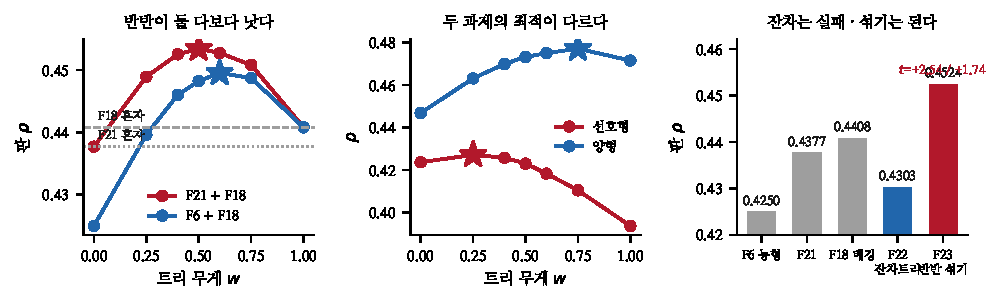
\includegraphics[width=\textwidth]{figs/mixing.pdf}
\caption{왼쪽 --- 반반이 둘 다보다 위. 가운데 --- 두 과제의 최적 무게가
다르다. 오른쪽 --- 잔차는 실패하고 섞기는 된다.}
\end{figure*}

\section{제안한 형태는 실패했다}

\begin{table}[t]
\centering\tsize
\caption{잔차 트리(F22).}
\begin{tabular}{lrrrr}
\toprule
& 판 & 선호형 & 양형 & 웹툰 \\
\midrule
F6 능형(바탕) & .4250 & .4140 & .4322 & .3891 \\
\textbf{F22 잔차트리} & \textbf{.4303} & .4038 & .4476 & .3662 \\
F21 & .4377 & .4236 & .4468 & .3926 \\
F18 배깅 & .4408 & .3936 & .4715 & .3361 \\
\bottomrule
\end{tabular}
\end{table}

\claimx{\textbf{둘 다보다 낮다}(F18 대비 $-$0.0099 · F21 대비 $-$0.0070).
자기 바탕 능형보다 $+$0.0053 오를 뿐이다.}{\textbf{능형이 뺀 뒤의 잔차에는
트리가 쓰던 것이 거의 안 남는다.} 노트 226이 ``빌리고 나서 가른다''를
제안했는데 \textbf{순서를 정해 주는 것 자체가 트리가 하던 일을 지웠다.}}

\section{따로 세워 섞으면 된다}

\begin{table}[t]
\centering\tsize
\caption{F21 과 F18 을 순위로 섞으면.}
\begin{tabular}{lrrr}
\toprule
트리 무게 $w$ & 판 & 선호형 & 양형 \\
\midrule
0.00 (F21 혼자) & .4377 & .4236 & .4468 \\
0.25 & .4489 & \textbf{.4271} & .4631 \\
\textbf{0.50} & \textbf{.4534} & .4230 & .4732 \\
0.75 & .4508 & .4104 & \textbf{.4771} \\
1.00 (F18 혼자) & .4408 & .3936 & .4715 \\
\bottomrule
\end{tabular}
\end{table}

\claimx{\textbf{두 예측의 유보 상관이 0.63$\sim$0.94 다} --- 웹툰 0.785 ·
애니 0.738 · 아이돌 0.627 · 세계애니 0.937. \textbf{같은 것을 안
잡는다.}}{그래서 섞이는 것이 있다. 정식화로 올려 다시 재니
\texttt{F23\_rankmix} 가 판 $+$0.4524 이고 \textbf{F21 대비
$+$0.0152($t{=}2.54$) · F18 대비 $+$0.0115($t{=}1.74$)로 둘 다 짝 1 SE
밖}이다.}

\begin{table}[t]
\centering\tsize
\caption{F23 이 하위 판마다 각각의 최고를 가져간다.}
\begin{tabular}{lrrr}
\toprule
& 선호형 & 양형 & 판 \\
\midrule
F21 & \textbf{.4236} & .4468 & .4377 \\
F18 배깅 & .3936 & \textbf{.4715} & .4408 \\
\textbf{F23 반반} & \textbf{.4237} & \textbf{.4711} & \textbf{.4524} \\
\bottomrule
\end{tabular}
\end{table}

\claimx{\textbf{선호형에서 F21 을 따라가고}($+$0.4237 대 $+$0.4236)
\textbf{양형에서 F18 을 따라간다}($+$0.4711 대 $+$0.4715). 어느 쪽도 안
잃는다.}{\textbf{노트 225가 판 하나 뒤에 숨겨 놓았던 0.055 짜리 반전이
여기서 값이 된다} --- 두 과제에서 이기는 모형이 다르니 섞으면 각 과제의
승자를 따라간다. \textbf{렌즈를 만든 것이 곧바로 이득이 됐다.}}

\section{무게를 안 골랐다}

\begin{table}[t]
\centering\tsize
\caption{안쪽 분할을 다섯 번 옮기면(노트 216 규약).}
\begin{tabular}{lrrrr}
\toprule
분할 & $w{=}0.4$ & $w{=}0.5$ & $w{=}0.6$ & 최고 \\
\midrule
.60 & .5412 & \textbf{.5418} & .5405 & 0.5 \\
.65 & .5385 & \textbf{.5392} & .5382 & 0.5 \\
.70 & .5455 & \textbf{.5457} & .5454 & 0.5 \\
.75 & .5412 & \textbf{.5422} & .5421 & 0.5 \\
.80 & .5359 & .5378 & \textbf{.5379} & 0.6 \\
\midrule
\multicolumn{4}{l}{최빈} & \textbf{0.5 (4/5)} \\
\bottomrule
\end{tabular}
\end{table}

\claimx{\textbf{다섯 분할 중 넷이 $w{=}0.5$ 를 고른다} --- 노트 216의
안정성 기준을 통과한다. 유보를 한 번도 안 봤다.}{\textbf{그리고 0.5 는
대칭 기본값이다} --- 고른 것이라기보다 \emph{안 고른} 것에 가깝다. 두
과제의 최적이 각각 0.25 와 0.75 인데 그 중간을 쓰는 것이므로, \textbf{어느
과제에도 맞추지 않은 무게다.}}

\begin{table}[t]
\centering\tsize
\caption{남은 것.}
\begin{tabular}{ll}
\toprule
\textbf{과제별 무게} & 선호형 0.25 · 양형 0.75 --- 갈라 쓸 것인가 \\
\textbf{셋째} & F6 · F9 를 더 섞으면 더 오르나 \\
잔차 실패 & 왜 순서를 정하면 지워지나 \\
\bottomrule
\end{tabular}
\end{table}

첫 줄이 값이 크고 위험하다. 두 과제의 최적 무게가 0.25 와 0.75 로 갈리고,
과제별로 쓰면 선호형 $+$0.4271 · 양형 $+$0.4771 로 \textbf{합쳐서
$+$0.4574} 가 된다($+$0.0050). \textbf{그런데 그 무게 둘을 유보에서
읽으면 엿보기다} --- 안쪽에서 과제별로 따로 고를 수 있는지, 그리고 그
선택이 노트 216의 안정성을 통과하는지를 먼저 봐야 한다. \textbf{과제가
둘이면 안쪽 표본도 둘로 갈리므로 각 곡면이 더 평평해질 것이고}, 노트 216이
잡은 바로 그 함정(평평한 곡면에서 최댓값을 고르면 잡음을 고른다)에 걸릴
공산이 크다.

\end{document}
